\documentclass[12pt]{article}

\usepackage[a4paper, margin=1in]{geometry}
\usepackage{fancyhdr}
\usepackage{titling}
\usepackage{babel}[latvian]
\usepackage{graphicx}
\usepackage{float}
\usepackage{dirtytalk}
\usepackage{gensymb}

\newlength\tindent
\setlength{\tindent}{\parindent}
\setlength{\parindent}{0pt}
\renewcommand{\indent}{\hspace*{\tindent}}

\fancypagestyle{plain}{
  \fancyhf{}
  \fancyhead[R]{ Andrejs Cvečkovskis \\ ac24005 \\ Kurss Zinātniskā programmēšana fiziķiem}
  \renewcommand{\headrulewidth}{0pt}
}

\title{\vspace{-1cm}\centering Laboratorijas darba \\[1ex] \large \say{Akselerometra datu apstrāde - Integrēšana un statistiskie aprēķini} \\ Protokols \vspace{-6em}}
\author{}
\date{}  
\begin{document}
\maketitle

\section*{Brīvās krišanas paātrinājuma g noteikšana}

1. Attēlot grafiski visas trīs paātrinājuma komponentes un brīvās krišanas paātrinājumu atkarībā no laika.
\begin{center}
    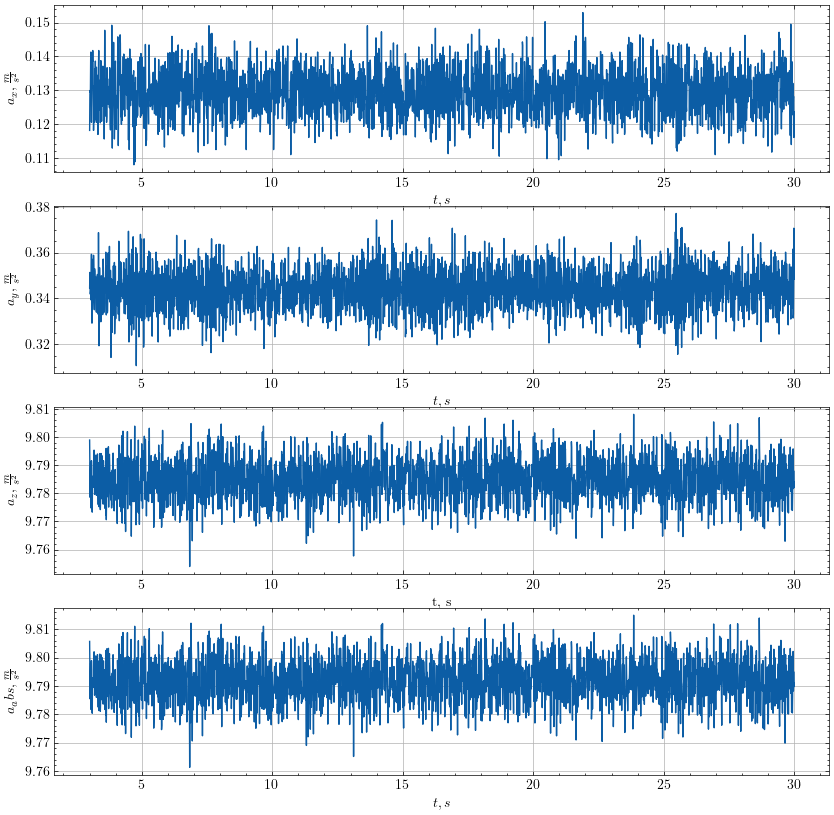
\includegraphics[width=1\textwidth]{Brīvās krišanas paātrinājuma g noteikšana1.png}
\end{center}

2.	Kāda ir vidējā vērtība brīvās krišanas paātrinājuma mērījumiem?

\indent \textbf{Atbilde:} Brīvās krišanas paātrinājuma vidējā vērtība - 9.791829491195932 $\frac{m}{s^2}$

3.	Kāda ir standartnovirze brīvās krišanas paātrinājuma mērījumiem?

\indent \textbf{Atbilde:} Brīvās krišanas paātrinājuma standartnovirze - 0.007389507201454131 $\frac{m}{s^2}$

4.	Attēlot grafiski histogrammu paātrinājuma komponenšu un brīvās krišanas paātrinājuma mērījumiem.
\begin{center}
    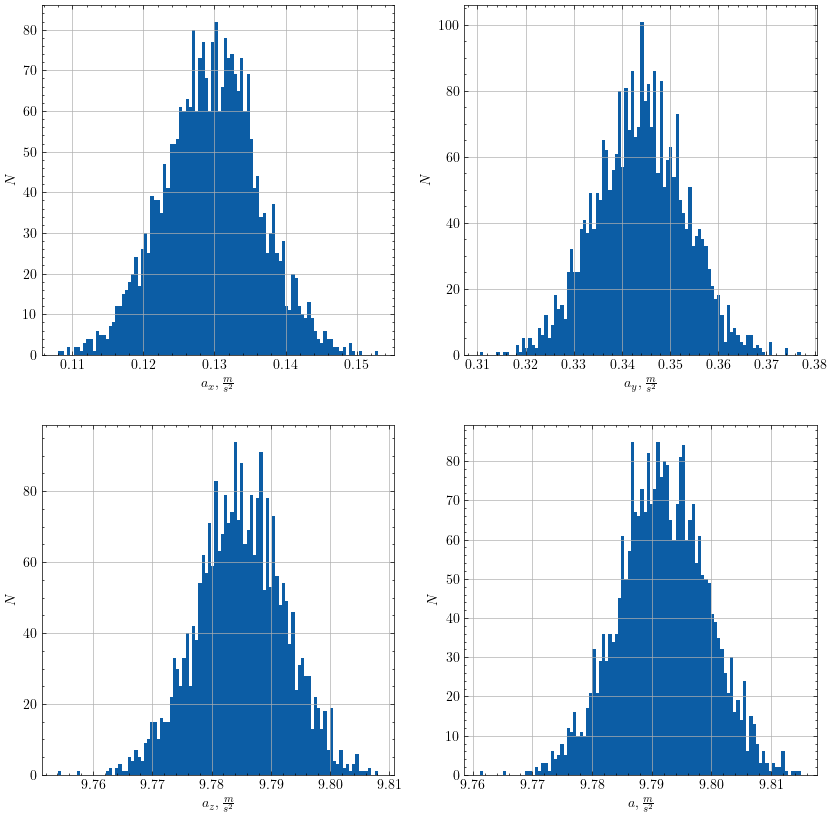
\includegraphics[width=1\textwidth]{Brīvās krišanas paātrinājuma g noteikšana2.png}
\end{center}

\begin{center}
    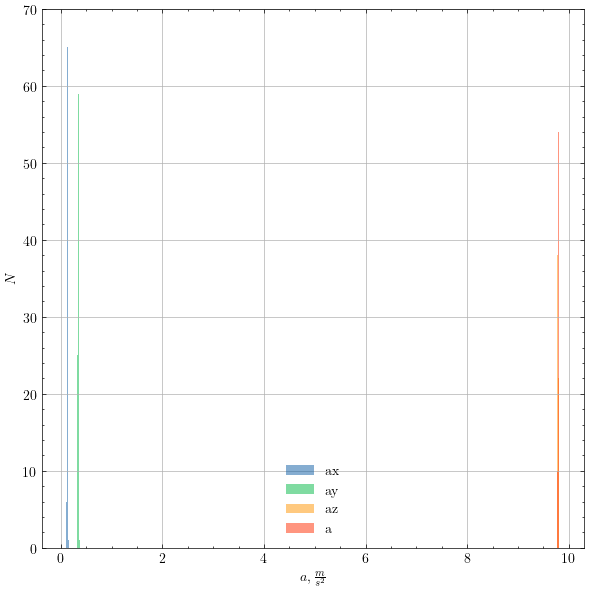
\includegraphics[width=1\textwidth]{Brīvās krišanas paātrinājuma g noteikšana3.png}
\end{center}

5.	Salīdzināt izmērīto brīvās krišanas paātrinājuma vērtību ar reālo. Komentēt rezultātus un kļūdu cēloņus.

\indent \textbf{Atbilde:} Izmērītā brīvās krišanas paātrinājuma vērtība, 9.79183 $\frac{m}{s^2}$, ir nedaudz zemāka nekā Rīgas reģionā noteiktais lokālais vērtējums – 9.81648 $\frac{m}{s^2}$ \cite{aleksejenko2012}. Šī nelielā atšķirība, aptuveni 0.02465 $\frac{m}{s^2}$, var rasties vairāku iemeslu dēļ, piemēram, MEMS akselerometri, kādi tiek izmantoti iPhone 15 Pro, ir jutīgi pret kalibrācijas kļūdām. Pat nelielas sistēmas īpašības un orientācijas neatbilstības var novest pie nelielām, bet sistemātiskām novirzēm. Apkārtējās vides vibrācijas un nelielas kustības varēja ietekmēt mērījumus.

6.	Vai brīvās krišanas paātrinājuma mērījumos novērojams sensora drifts? Pamatot atbildi!

\indent \textbf{Atbilde:} Vidējā vērtība laika gaitā būtiski nemainās un mērījumu izkliede saglabājas ap līdzīgu līmeni (histogrammas ir samērā simetriskas, bet laika diapazonā neparādās sistemātiska vērtību nobīde). Ja sensora drifts būtu izteikts, redzētu pakāpenisku un nepārtrauktu vidējās vērtības maiņu (piemēram, no 9.76 $\frac{m}{s^2}$² uz 9.79 $\frac{m}{s^2}$ virzienā vienā virzienā), taču šādas tendences grafikā nav novērojamas. Tādēļ var secināt, ka brīvās krišanas paātrinājuma mērījumos sensora drifta nav vai arī ir pietiekami mazs, lai neizpaustos redzamā laika diapazonā.

\subsection*{Uzrakstītais kods}
\begin{center}
    \begin{verbatim}
t = filtered_accelerometer.index
        
g_x = filtered_accelerometer['ax']
g_y = filtered_accelerometer['ay']
g_z = filtered_accelerometer['az']
g_abs = filtered_accelerometer['a']
        
fig, ax = plt.subplots(4, 1, figsize=(10, 10))
ax[0].plot(t, g_x, label='ax')
ax[0].set_ylabel(r'$a_x, \frac{m}{s^2}$')
ax[0].set_xlabel(r'$t, s$')
ax[0].grid(True)
        
ax[1].plot(t, g_y, label='ay')
ax[1].set_ylabel(r'$a_y, \frac{m}{s^2}$')
ax[1].set_xlabel(r'$t, s$')
ax[1].grid(True)
        
ax[2].plot(t, g_z, label='az')
ax[2].set_ylabel(r'$a_z, \frac{m}{s^2}$')
ax[2].set_xlabel(r't, s')
ax[2].grid(True)
        
ax[3].plot(t, g_abs, label='a')
ax[3].set_ylabel(r'$a_abs, \frac{m}{s^2}$')
ax[3].set_xlabel(r'$t, s$')
ax[3].grid(True)
        
g_mean = g_abs.mean()
print('Vidējā vērtība:', g_mean)
        
        
std = np.std(g_abs, ddof=1)
print('Standartnovirze:', std)
        
fig, ax = plt.subplots(2, 2, figsize=(10, 10))
ax[0, 0].hist(g_x, bins=100)
ax[0, 0].set_xlabel(r'$a_x, \frac{m}{s^2}$')
ax[0, 0].set_ylabel(r'$N$')
ax[0, 0].grid(True)
        
ax[0, 1].hist(g_y, bins=100)
ax[0, 1].set_xlabel(r'$a_y, \frac{m}{s^2}$')
ax[0, 1].set_ylabel(r'$N$')
ax[0, 1].grid(True)
        
ax[1, 0].hist(g_z, bins=100)
ax[1, 0].set_xlabel(r'$a_z, \frac{m}{s^2}$')
ax[1, 0].set_ylabel(r'$N$')
ax[1, 0].grid(True)
        
ax[1, 1].hist(g_abs, bins=100)
ax[1, 1].set_xlabel(r'$a, \frac{m}{s^2}$')
ax[1, 1].set_ylabel(r'$N$')
ax[1, 1].grid(True)
        
plt.show()

fig, ax = plt.subplots(1, 1, figsize=(7, 7))
ax.hist(g_x, bins=100, alpha=0.5, label='ax')
ax.hist(g_y, bins=100, alpha=0.5, label='ay')
ax.hist(g_z, bins=100, alpha=0.5, label='az')
ax.hist(g_abs, bins=100, alpha=0.5, label='a')
ax.set_ylim(0, 70)
ax.set_xlabel(r'$a, \frac{m}{s^2}$')
ax.set_ylabel(r'$N$')
ax.legend()
ax.grid(True)
plt.show()
    \end{verbatim}
\end{center}

\newpage
\section*{Zemes rotācijas leņķiskā ātruma $\omega$ noteikšana}

1.	Attēlot grafiski visas trīs leņķiskā ātruma komponentes un Zemes rotācijas leņķisko ātrumu atkarībā no laika.

\begin{center}
    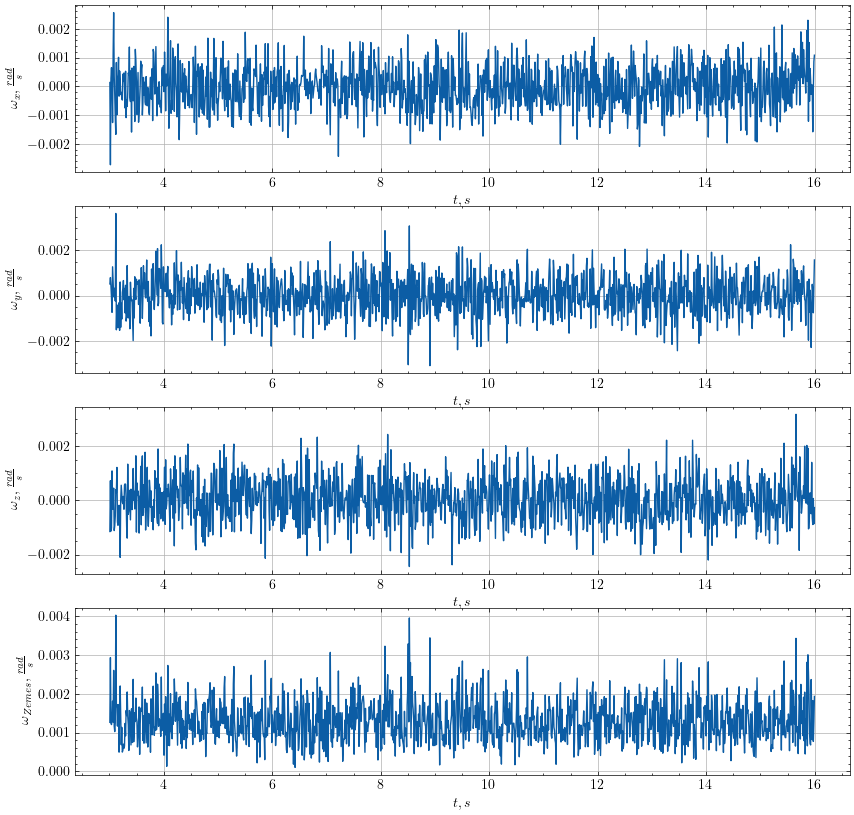
\includegraphics[width=1\textwidth]{Zemes rotācijas leņķiskā ātruma noteikšana1.png}
\end{center}

2.	Kāda ir vidējā vērtība Zemes rotācijas leņķiskā ātruma mērījumiem?

\indent \textbf{Atbilde:} Vidējā vērtība Zemes rotācijas leņķiskā ātruma mērījumiem - 0.001306073872471275 $\frac{rad}{s}$

3.	Kāda ir standartnovirze Zemes rotācijas leņķiskā ātruma mērījumiem?

\indent \textbf{Atbilde:} Zemes rotācijas leņķiskā ātruma standartnovirze - 0.0005414114764589375 $\frac{rad}{s}$

4.	Attēlot grafiski histogrammu leņķiskā ātruma komponenšu un Zemes rotācijas leņķiskā ātruma mērījumiem.

\begin{center}
    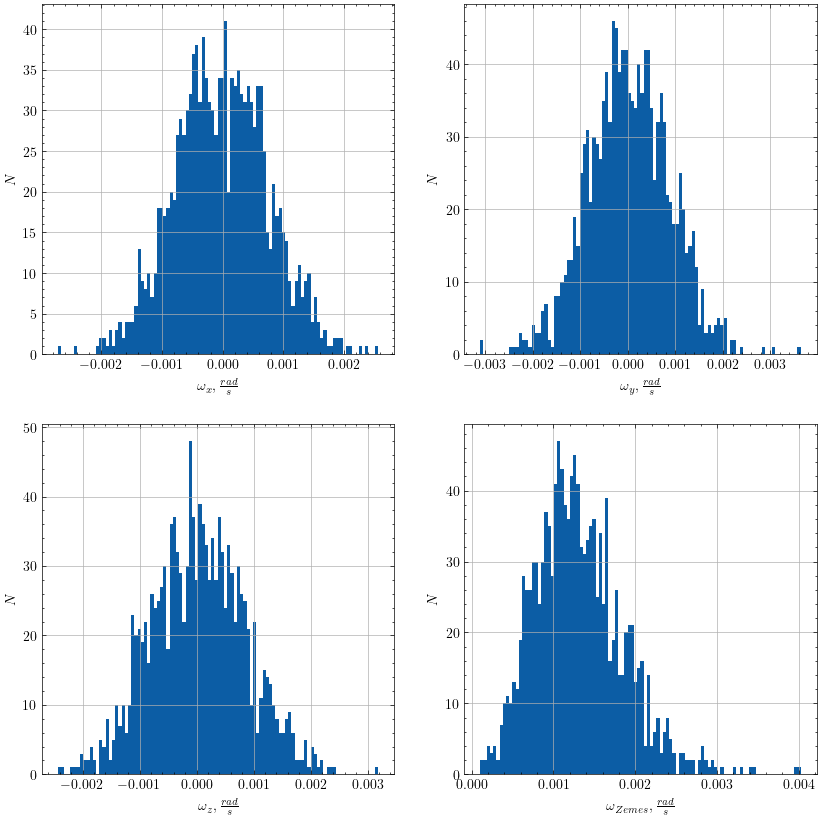
\includegraphics[width=1\textwidth]{Zemes rotācijas leņķiskā ātruma noteikšana2.png}
    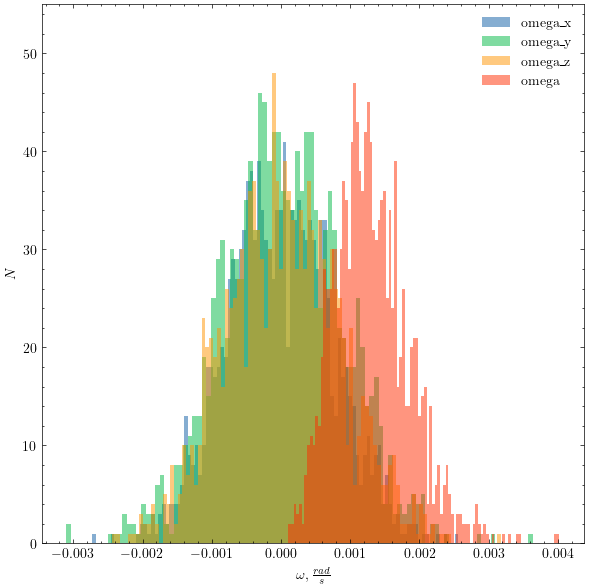
\includegraphics[width=1\textwidth]{Zemes rotācijas leņķiskā ātruma noteikšana3.png}
\end{center}

5.	Salīdzināt izmērīto Zemes rotācijas leņķiskā ātrumā vērtību ar reālo. Komentēt rezultātus un kļūdu cēloņus.

\indent \textbf{Atbilde:} Izmērītā Zemes rotācijas leņķiskā ātruma vidējā vērtība (aptuveni 0.001306 $\frac{rad}{s}$) ir aptuveni 17–18 reizes lielāka par reālo Zemes rotācijas ātrumu, kas ir 7.292 $\cdot 10^5 \frac{rad}{s}$ \cite{earth_rotation_velocity}. Galvenie kļūdu cēloņi var būt ierīces lokālā kustība, vibrācijas no datora ventilatoriem vai orientācijas kļūda.

6.	Vai brīvās Zemes rotācijas leņķiskā ātruma mērījumos novērojams sensora drifts? Pamatot atbildi!

\indent \textbf{Atbilde:} Datos netiek novērota sistemātiska, pakāpeniska leņķiskā ātruma vērtības nobīde vienā virzienā. Lai gan vidējā vērtība ir ievērojami lielāka par reālo Zemes rotācijas ātrumu, šī atšķirība saglabājas salīdzinoši nemainīga visa mērījumu posma laikā.

\subsection*{Uzrakstītais kods}
\begin{center}
    \begin{verbatim}

t = filtered_gyroscope.index

omega_x = filtered_gyroscope['omega_x']
omega_y = filtered_gyroscope['omega_y']
omega_z = filtered_gyroscope['omega_z']
omega_abs = filtered_gyroscope['omega']

fig, ax = plt.subplots(4, 1, figsize=(10, 10))
ax[0].plot(t, omega_x, label='omega_x')
ax[0].set_ylabel(r'$\omega_{x}, \frac{rad}{s}$')
ax[0].set_xlabel(r'$t, s$')
ax[0].grid(True)

ax[1].plot(t, omega_y, label='omega_y')
ax[1].set_ylabel(r'$\omega_{y}, \frac{rad}{s}$')
ax[1].set_xlabel(r'$t, s$')
ax[1].grid(True)

ax[2].plot(t, omega_z, label='omega_z')
ax[2].set_ylabel(r'$\omega_{z}, \frac{rad}{s}$')
ax[2].set_xlabel(r'$t, s$')
ax[2].grid(True)

ax[3].plot(t, omega_abs, label='omega')
ax[3].set_ylabel(r'$\omega_{Zemes}, \frac{rad}{s}$')
ax[3].set_xlabel(r'$t, s$')
ax[3].grid(True)

plt.show()

omega_mean = omega_abs.mean()
print('Vidējā vērtība:', omega_mean)

std = np.std(omega_abs, ddof=1)
print('Standartnovirze:', std)

fig, ax = plt.subplots(2, 2, figsize=(10, 10))
ax[0, 0].hist(omega_x, bins=100)
ax[0, 0].set_xlabel(r'$\omega_{x}, \frac{rad}{s}$')
ax[0, 0].set_ylabel(r'$N$')
ax[0, 0].grid(True)

ax[0, 1].hist(omega_y, bins=100)
ax[0, 1].set_xlabel(r'$\omega_{y}, \frac{rad}{s}$')
ax[0, 1].set_ylabel(r'$N$')
ax[0, 1].grid(True)

ax[1, 0].hist(omega_z, bins=100)
ax[1, 0].set_xlabel(r'$\omega_{z}, \frac{rad}{s}$')
ax[1, 0].set_ylabel(r'$N$')
ax[1, 0].grid(True)

ax[1, 1].hist(omega_abs, bins=100)
ax[1, 1].set_xlabel(r'$\omega_{Zemes}, \frac{rad}{s}$')
ax[1, 1].set_ylabel(r'$N$')
ax[1, 1].grid(True)

plt.show()

fig, ax = plt.subplots(1, 1, figsize=(7, 7))
ax.hist(omega_x, bins=100, alpha=0.5, label='omega_x')
ax.hist(omega_y, bins=100, alpha=0.5, label='omega_y')
ax.hist(omega_z, bins=100, alpha=0.5, label='omega_z')
ax.hist(omega_abs, bins=100, alpha=0.5, label='omega')
ax.legend()
ax.set_ylim(0, 55)
ax.set_xlabel(r'$\omega, \frac{rad}{s}$')
ax.set_ylabel(r'$N$')

    \end{verbatim}
\end{center}

\newpage
\section*{Telefona pagrieziena leņķa noteikšana}

1.	Attēlot grafiski izmērīto telefona leņķisko ātrumu atkarībā no laika.

\begin{center}
    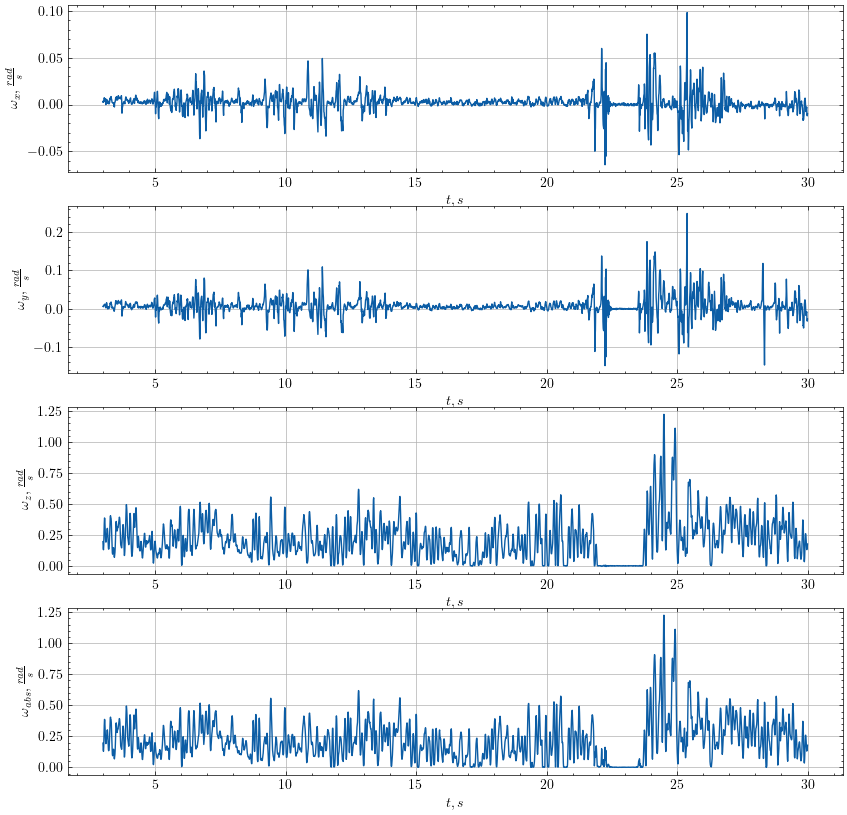
\includegraphics[width=1\textwidth]{Telefona pagrieziena leņķa noteikšana1.png}
\end{center}

2.	Attēlot grafiski telefona kopējo pagrieziena leņķi atkarībā no laika.

\begin{center}
    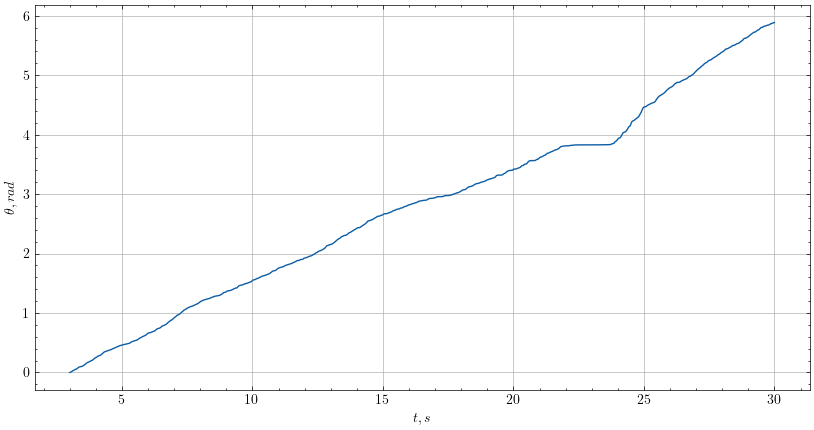
\includegraphics[width=1\textwidth]{Telefona pagrieziena leņķa noteikšana2.png}
\end{center}

3.	Kods telefona pagrieziena leņķa aprēķināšanai, izmantojot sensora datus.
\begin{center}
\begin{verbatim}
t = filtered_angle.index
dt = 0.01

angle = np.zeros(len(t))
for i in range(len(t)-1):
    angle[i+1] = angle[i] + filtered_angle['a'].iloc[i]*dt

angle_x_int = np.zeros(len(t))
angle_y_int = np.zeros(len(t))
angle_z_int = np.zeros(len(t))
for i in range(len(t)-1):
    angle_x_int[i+1] = angle_x_int[i] + filtered_angle['ax'].iloc[i]*dt
    angle_y_int[i+1] = angle_y_int[i] + filtered_angle['ay'].iloc[i]*dt
    angle_z_int[i+1] = angle_z_int[i] + filtered_angle['az'].iloc[i]*dt
\end{verbatim}
\end{center}
4.	Salīdzināt aprēķināto kopējo telefona pagrieziena leņķi ar reālo. Komentēt rezultātus un kļūdu cēloņus!

\indent \textbf{Atbilde:} Aprēķinātais kopējais pagrieziena leņķis (5.887781842843002 rad) ir samērā tuvs reālajam 360 $^{\circ}$ (2$\pi$ $\approx$ 6.283 rad) pagriezienam, tomēr redzama $\approx$ 0.395 rad (ap 23$^{\circ}$) novirze. Viens no galvenajiem kļūdu avotiem šajā gadījumā ir Eilera metodes izmantošana leņķa aprēķinā

\subsection*{Uzrakstītais kods}

\begin{center}
\begin{verbatim}

t = filtered_angle.index

a_x = filtered_angle['ax']
a_y = filtered_angle['ay']
a_z = filtered_angle['az']

a_abs = filtered_angle['a']

fig, ax = plt.subplots(4, 1, figsize=(10, 10))
ax[0].plot(t, a_x, label='a_x')
ax[0].set_ylabel(r'$\omega_{x}, \frac{rad}{s}$')
ax[0].set_xlabel(r'$t, s$')
ax[0].grid(True)

ax[1].plot(t, a_y, label='a_y')
ax[1].set_ylabel(r'$\omega_{y}, \frac{rad}{s}$')
ax[1].set_xlabel(r'$t, s$')
ax[1].grid(True)

ax[2].plot(t, a_z, label='a_z')
ax[2].set_ylabel(r'$\omega_{z}, \frac{rad}{s}$')
ax[2].set_xlabel(r'$t, s$')
ax[2].grid(True)

ax[3].plot(t, a_abs, label='a')
ax[3].set_ylabel(r'$\omega_{abs}, \frac{rad}{s}$')
ax[3].set_xlabel(r'$t, s$')
ax[3].grid(True)

plt.show()

t = filtered_angle.index
dt = 0.01

angle = np.zeros(len(t))
for i in range(len(t)-1):
    angle[i+1] = angle[i] + filtered_angle['a'].iloc[i]*dt

angle_x_int = np.zeros(len(t))
angle_y_int = np.zeros(len(t))
angle_z_int = np.zeros(len(t))
for i in range(len(t)-1):
    angle_x_int[i+1] = angle_x_int[i] + filtered_angle['ax'].iloc[i]*dt
    angle_y_int[i+1] = angle_y_int[i] + filtered_angle['ay'].iloc[i]*dt
    angle_z_int[i+1] = angle_z_int[i] + filtered_angle['az'].iloc[i]*dt

fig, ax = plt.subplots(1, 1, figsize=(10, 5))
ax.plot(t, angle, label='angle')
ax.set_ylabel(r'$\theta, rad$')
ax.set_xlabel(r'$t, s$')
ax.grid(True)

plt.show()

\end{verbatim}
\end{center}

\section*{Telefona pārvietojuma noteikšana}

1.	Attēlot grafiski izmērīto telefona paātrinājuma komponentes atkarībā no laika.

\begin{center}
    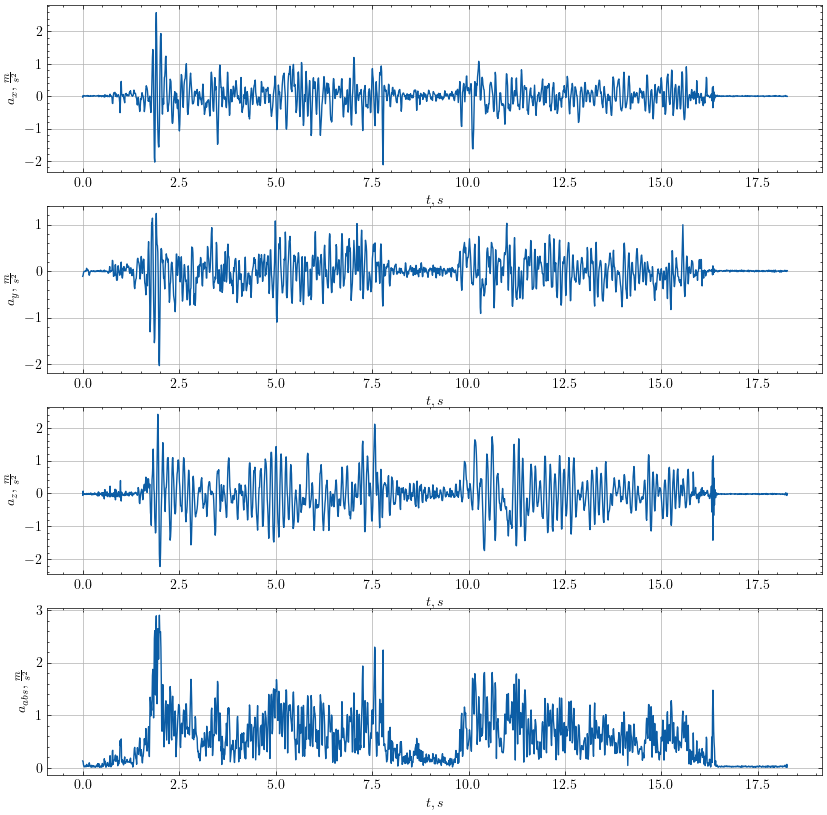
\includegraphics[width=1\textwidth]{Telefona pārvietojuma noteikšana1.png}
\end{center}

2.	Attēlot grafiski telefona ātruma komponentes atkarībā no laika.

\begin{center}
    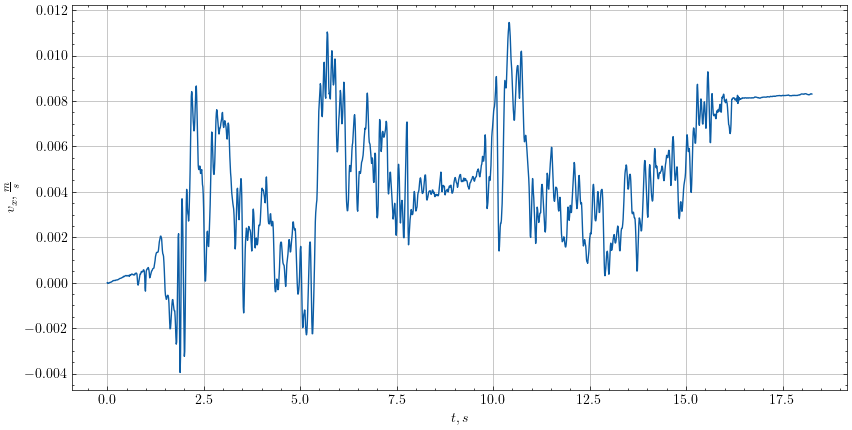
\includegraphics[width=1\textwidth]{Telefona pārvietojuma noteikšana2.png}
\end{center}

3.	Attēlot grafiski telefona pārvietojuma komponentes atkarībā no laika.

\begin{center}
    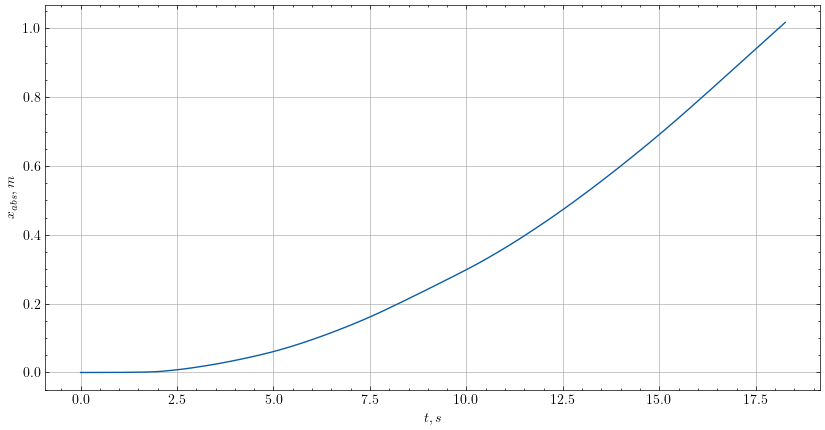
\includegraphics[width=1\textwidth]{Telefona pārvietojuma noteikšana3.png}
\end{center}

4.	Kods telefona ātruma un koordinātas aprēķināšanai, izmantojot sensora datus.

\begin{center}
    \begin{verbatim}
        t = df_acceleration_without_g.index
        
        a_abs = df_acceleration_without_g['omega']
        
        dt = 0.001
        
        v_abs = np.zeros(len(t))
        for i in range(len(t)-1):
            v_abs[i+1] = v_abs[i] + a_abs.iloc[i]*dt
        
        x_abs = np.zeros(len(t))
        for i in range(len(t)-1):
            x_abs[i+1] = x_abs[i] + v_abs[i]*dt
    \end{verbatim}
\end{center}

5.	Kods telefona maksimālā ātruma aprēķināšanai.

\begin{center}
    \begin{verbatim}
        max_v = v_abs.max()
        print('Maksimālais ātrums:', max_v)
    \end{verbatim}  
\end{center}

6.	Salīdzināt aprēķināto kopējo telefona pārvietojumu ar reālo. Komentēt rezultātus un kļūdu cēloņus!

\indent \textbf{Atbilde:} Aprēķinātais telefona kopējais pārvietojums (1.0174 m) ir ļoti tuvs reālajai $\approx$ 1 m distancei. Novirze ap 1–2 cm šādā eksperimentā ar viedtālruņa iebūvētiem sensoriem ir uzskatāma par samērā labu rezultātu. Kļūdas galvenokārt rodas no dubultās integrēšanas, telefona pārvietošanas trajektorijas un vertikālās kustības un Eilera metodes ierobežojumiem.

\subsection*{Uzrakstītais kods:}

\begin{center}

\begin{verbatim}

print(filtered_acceleration_without_g)

t = df_acceleration_without_g.index

a_x = df_acceleration_without_g['omega_x']
a_y = df_acceleration_without_g['omega_y']
a_z = df_acceleration_without_g['omega_z']

a_abs = df_acceleration_without_g['omega']

dt = 0.001

v_x = np.zeros(len(t))
for i in range(len(t)-1):
    v_x[i+1] = v_x[i] + a_x.iloc[i]*dt

v_y = np.zeros(len(t))
for i in range(len(t)-1):
    v_y[i+1] = v_y[i] + a_y.iloc[i]*dt

v_z = np.zeros(len(t))
for i in range(len(t)-1):
    v_z[i+1] = v_z[i] + a_z.iloc[i]*dt

v_abs = np.zeros(len(t))
for i in range(len(t)-1):
    v_abs[i+1] = v_abs[i] + a_abs.iloc[i]*dt

x_abs = np.zeros(len(t))
for i in range(len(t)-1):
    x_abs[i+1] = x_abs[i] + v_abs[i]*dt

fig, ax = plt.subplots(4, 1, figsize=(10, 10))

ax[0].plot(t, a_x, label='a_x')
ax[0].set_ylabel(r'$a_x, \frac{m}{s^2}$')
ax[0].set_xlabel(r'$t, s$')
ax[0].grid(True)

ax[1].plot(t, a_y, label='a_y')
ax[1].set_ylabel(r'$a_y, \frac{m}{s^2}$')
ax[1].set_xlabel(r'$t, s$')
ax[1].grid(True)

ax[2].plot(t, a_z, label='a_z')
ax[2].set_ylabel(r'$a_z, \frac{m}{s^2}$')
ax[2].set_xlabel(r'$t, s$')
ax[2].grid(True)

ax[3].plot(t, a_abs, label='a')
ax[3].set_ylabel(r'$a_{abs}, \frac{m}{s^2}$')
ax[3].set_xlabel(r'$t, s$')
ax[3].grid(True)

plt.show()

fig, ax = plt.subplots(1, 1, figsize=(10, 5))
ax.plot(t, v_x, label='v_x')
ax.set_ylabel(r'$v_x, \frac{m}{s}$')
ax.set_xlabel(r'$t, s$')
ax.grid(True)

plt.show()

fig, ax = plt.subplots(1, 1, figsize=(10, 5))
ax.plot(t, x_abs, label='x_abs')
ax.set_ylabel(r'$x_{abs}, m$')
ax.set_xlabel(r'$t, s$')
ax.grid(True)

plt.show()

max_v = v_abs.max()
print('Maksimālais ātrums:', max_v)
    
\end{verbatim}

\end{center}

\section*{Papilduzdevums – galda tenisa bumbiņas atlēkšanas augstuma noteikšana}

Telefons tika novietots uz galda, un pingponga bumbiņa tika palaista no aptuveni 30 cm augstuma, lai varētu reģistrēt vairākus atlēcienus. \say{Acceleration (without g)} datos tika fiksēti sadursmju maksimumi, kas identificēti ar funkciju find peaks. Mērot laiku starp šiem maksimumiem, tika aprēķināts katra atsitiena maksimālais augstums, iegūstot atsperīguma koeficientu $\approx$ \textbf{1.0339}, kas pārsniedz 1 un tāpēc ir fizikāli neticams. Šo neatbilstību rada sensora troksnis, kalibrēšanas neprecizitātes, nelielas galda (telefona/datora) vibrācijas vai nepilnīga gravitācijas konstante, kas izraisa nelielas laika nobīdes, kas palielina aprēķināto atsitiena augstumu. Ar precīzāku filtrēšanu un stabilāku iestatījumu izmērītais koeficients, visticamāk, samazinātos zem 1, kas atbilstu sagaidāmajiem enerģijas zudumiem.

\begin{center}
    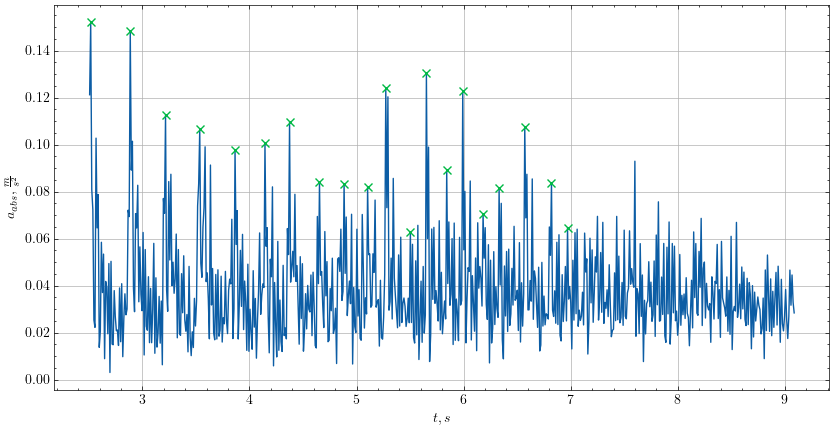
\includegraphics[width=1\textwidth]{Papilduzdevums – galda tenisa bumbiņas atlēkšanas augstuma noteikšana1.png}
\end{center}


\begin{center}
    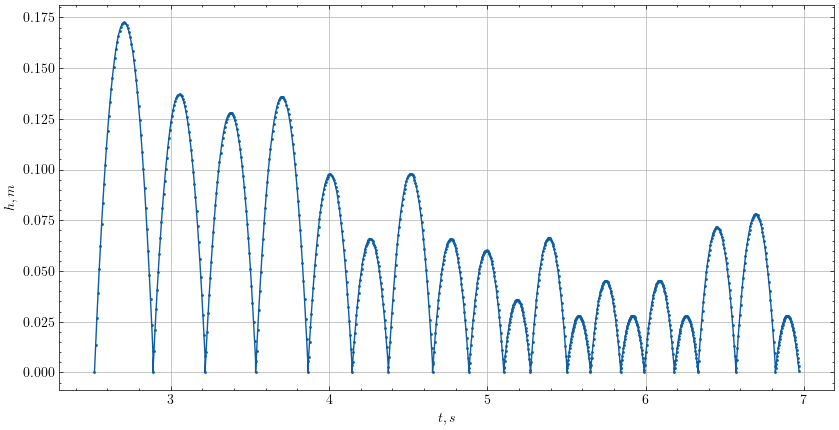
\includegraphics[width=1\textwidth]{Papilduzdevums – galda tenisa bumbiņas atlēkšanas augstuma noteikšana2.png}
\end{center}

\subsection*{Uzrakstītais kods}

\begin{center}

\begin{verbatim}

t = filtered_ball.index

a_x = filtered_ball['ax']
a_y = filtered_ball['ay']
a_z = filtered_ball['az']
a_abs = filtered_ball['a']

# use scipy.signal.find_peaks to find the peaks using the numpy values
peaks, _ = find_peaks(a_abs.values, height=0.059, distance=13)
# first 20 peaks
peaks = peaks[:20]
# add the peaks to the plot
fig, ax = plt.subplots(1, 1, figsize=(10, 5))
ax.plot(t, a_abs, label='a_abs')
ax.plot(t.to_numpy()[peaks], a_abs.values[peaks], 'x', label='peaks')
ax.set_ylabel(r'$a_{abs}, \frac{m}{s^2}$')
ax.set_xlabel(r'$t, s$')
ax.grid(True)
plt.show()

# calculate the time difference
between the peaks (using the first 20 peaks as before)
dt = np.diff(t.to_numpy()[peaks])

# Calculate the bounce heights starting with h0 as the initial height
h_0 = 0.3
v0 = 0
g = 9.81 # m/s^2
h_values = []  # starting height
time_values = []  # time values

# calculate h 
for idx, delta_t in enumerate(dt):
    # calculate the initial velocity
    acc = a_abs.values[peaks[idx]] + g
    v0 = np.abs(acc*delta_t/2)
    # calculate the height from one peak to the next
    t_local = np.linspace(0, delta_t, 50)
    t_global = np.linspace(t.to_numpy()[peaks[idx]], t.to_numpy()[peaks[idx+1]], 50)
    h = v0*t_local - 0.5*g*t_local**2
    h_values.extend(h)
    time_values.extend(t_global)


# plot the bounce heights over time (using the first 20 peaks)
fig, ax = plt.subplots(1, 1, figsize=(10, 5))
ax.plot(time_values, h_values, '-o', label='Bounce Heights', markersize=1)
ax.set_ylabel(r'$h, m$')
ax.set_xlabel(r'$t, s$')
ax.grid(True)
plt.show()

# calculate the coefficient
\end{verbatim}
    
\end{center}

\renewcommand{\refname}{Izmantotā literatūra}
\bibliographystyle{plain}
\bibliography{bib}


\end{document}
